\chapter{Introduction}
\label{chap:Intro}
\par
Airports often lack insight about how many passengers are expected on various security checks, arrival/departure gates, etc. As a consequence of these inaccurate predictions, they are commonly either understaffed or overstaffed. This inefficient resource management increases the airport’s expenses, as well as passenger waiting time. As this can be generally attributed to difficulties obtaining and processing data, more clever approaches need to be utilised.\newline

\par
To deal with this problem, the company Blip Systems has sensors installed at various locations throughout the airport layout. The sensors are capable of recording the signal strength of mobile devices using Wi-Fi or Bluetooth and, therefore, provide a possibility to model passenger flow around congested areas. Unfortunately, the data these sensors detect are not trivial to interpret, as there is complexity around different patterns of individuals, as well as around detecting "outliers" (e.g. airport personnel, incorrect measurements, signal noise, etc.), which are not relevant for the airport’s insight of resource management.\newline

\par
The implementation currently in use by Blip Systems requires too many resources in the process of taking the data from the Raw Sensor Records to System Validation. They have manually set up rules for calibrating the data and over 100 rules for modelling the data, as illustrated in \cref{fig:strategy_of_blip}.\newline
\begin{figure}[H]
	\centering
	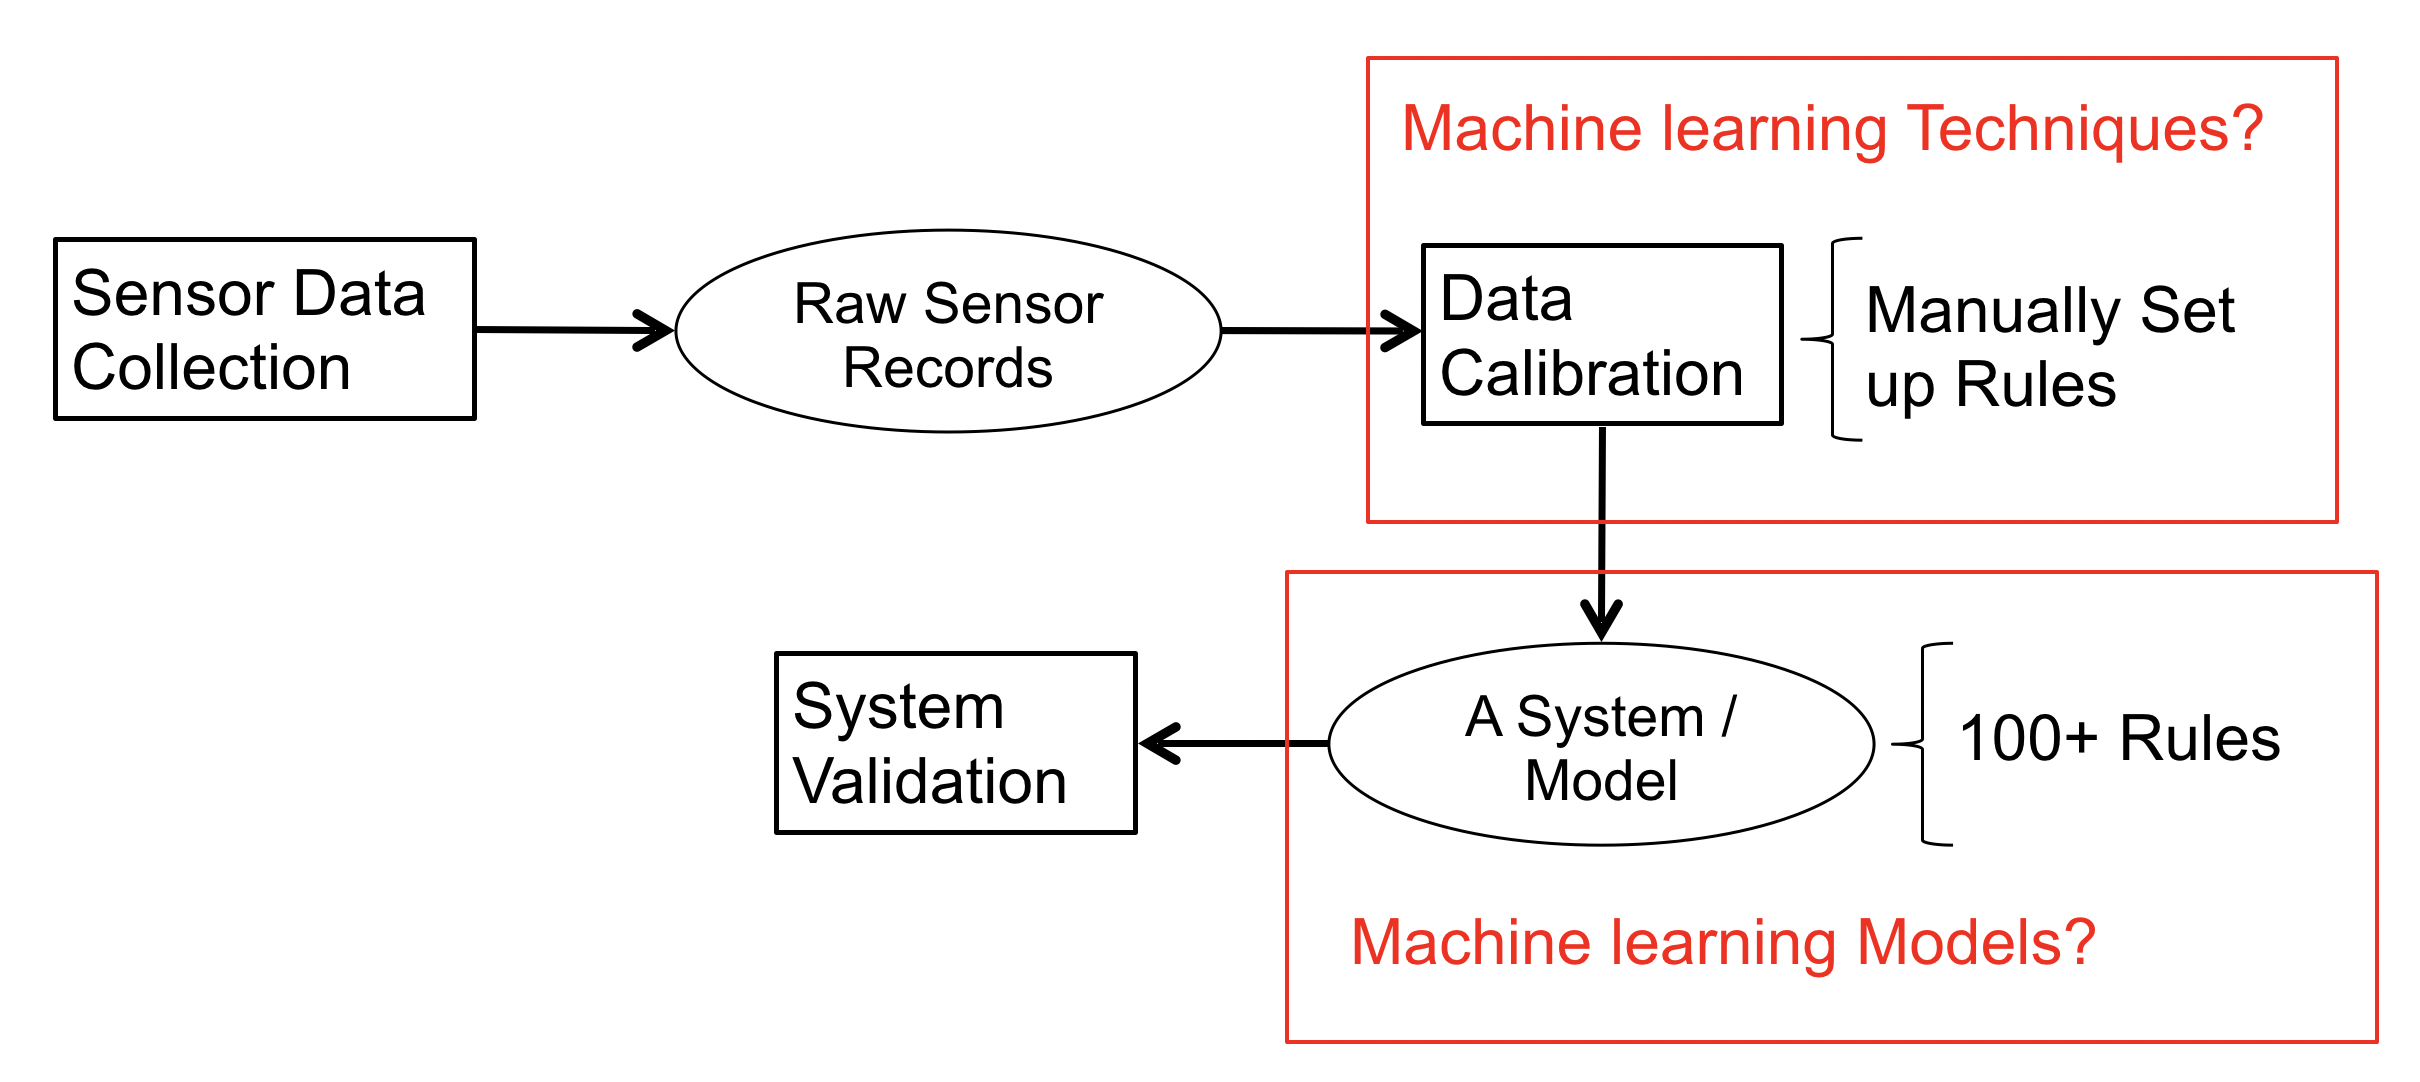
\includegraphics[width=0.75\textwidth]{related_work.png}
	\caption{The-State-of-the-Art Strategy of Blip Systems A/S}
	\label{fig:strategy_of_blip}
\end{figure}

\par
This project focuses on exploring machine learning techniques to distinguish and classify the raw sensor data of mobile devices. We should provide a more efficient solution for data calibration and modelling without the need for fine-grained manually created logic. Rather than analysing the data of the entire airport, a specific area - the arrival gate - was chosen.\newline

\par
The involved data set is a set of measurements collected from the sensors placed throughout the area. The raw, multidimensional data comes with intricacies of wireless signals and mobile device, such as variance in signal strength or edge cases create by different device usage patterns. This poses a significant challenge for data processing, which is why the data will need to be modelled to both represent the behaviour of passengers appropriately, as well as conform to the constraints of machine learning techniques to be utilised. \newline

\par
To achieve the goal of this project, the following methods will be used:

We will conduct our initial experiments using Label propagation as a baseline method with the focus on modelling the similarities among data in form of multivariate times series. The baseline will serve us as a simple method to get some initial results and help us to better understand the data, as well as to decide on further direction.
Afterwards, we will experiment with Decision Trees, a feature-centric technique, which will demand features to be extracted from the data (feature engineering).
Finally, the last stage will require a more complex, deep learning model such as Convolutional Neural Networks, where the objective will be to discover and learn patterns in the data automatically.